\documentclass{article}

% Packages
\usepackage[utf8]{inputenc}
\usepackage[english]{babel}

\usepackage{amsthm}
\usepackage{amsfonts}
\usepackage{amssymb}
\usepackage{graphicx}
\usepackage{caption}

% Theorems
\theoremstyle{definition}

\newtheorem{definition}{Definition}[section]
\newtheorem{proposition}{Proposition}[section]

\theoremstyle{remark}

\newtheorem*{remark}{Remark}
\newtheorem*{theorem}{Theorem}

% Commands
\newcommand{\func}[3]{#1:#2\rightarrow#3}
\newcommand{\reqfunc}[2]{#1:#2\rightarrow\mathbb{B}}
\newcommand{\reqop}[2]{\mathbf{Req}_{#1}(#2)}

\newcommand{\path}[2]{\mathbf{Path}^{#2}_{#1}}
\newcommand{\pathall}[1]{\mathbf{Path}_{#1}}
\newcommand{\cyclepath}[1]{\mathbf{Cycle}_{#1}}

\newcommand{\labeledarrow}[1]{\stackrel{#1}{\rightarrow}}

\newcommand{\setbuild}[3]
{
	\{\hspace{0.05in} 
	#1 \in #2 \hspace{0.05in} 
	| \hspace{0.05in}#3\hspace{0.05in}
	\}	
}

% Preamble
\title{Scala Job Scheduler}
\date{February 2018}

% --------------------------------------------------------------------------
\begin{document}
	
	% Title page
	\pagenumbering{gobble}
	\maketitle
	
	% Table of contents
	\newpage
	\tableofcontents
	
	% Begin main document
	\newpage
	\pagenumbering{arabic}
	
	\section{Introduction}
	
	\indent
	
	The aim of this project is to design an optimal scheduling algorithm for a scalable computing cloud, where computing resources are dynamically allocated to meet the demands of an inhomogeneous set of consumers. Resources are not uniformly distributed, geographically or otherwise, as the nodes comprising the cloud are of variable type and processing power. Clients will submit job specifications (indicating the number and type of cores, ideal network topology, required run time, etc.) to the scheduler, which should designate a time to run and a cluster of nodes that adheres to the specification. The algorithm should maximize throughput (efficient use of resources) while maintaining fairness, with wait times minimal and consistent between jobs that place similar demands on the system.
	
	In order to build an algorithm capable of operating on a complex, heterogeneous system of resources and consumers, we must consider the process from an abstract yet granular point of view. In an attempt to do so we have defined the system in terms of simple mathematical objects, and constructed an algebra over those objects to describe their interaction. By decomposing the scheduling process into its constituent parts, we were able to describe each component of the process in terms of this algebra and thus devise a mathematical model for the process as a whole. 
	
	Due to the difficulty of processing such a dynamic, diverse system (given the sheer number of factors to account for), we elected to confront the problem with a reinforcement learning algorithm built on the aforementioned model. The algorithm is highly dependent on the system's partitioning into measurable (numerically describable) components, and typifying these components for efficient processing - thus the focus on separability and producing quantifiable descriptors of the system. What follows is a detailed specification of the resultant scheduling paradigm: first of the environment and scheduling process, component by component, and then the construction of the reinforcement model from those components.
	
	1. General Process:
	
	\begin{figure1}
	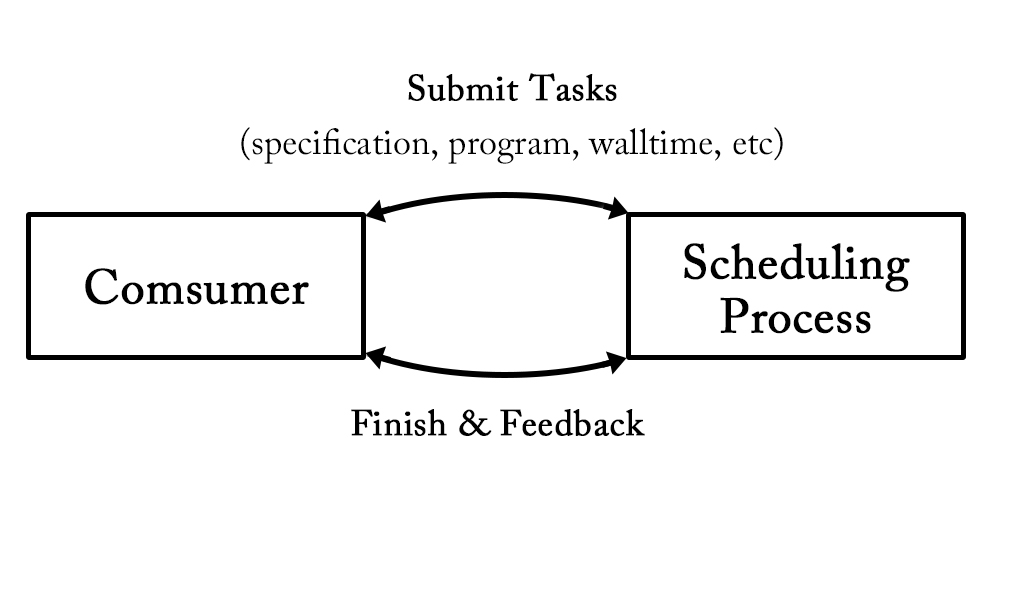
\includegraphics[width=1.0\textwidth]{Intro1.jpg}
	\caption{}
	\end{figure1}
	
	
	
	\begin{figure2}
	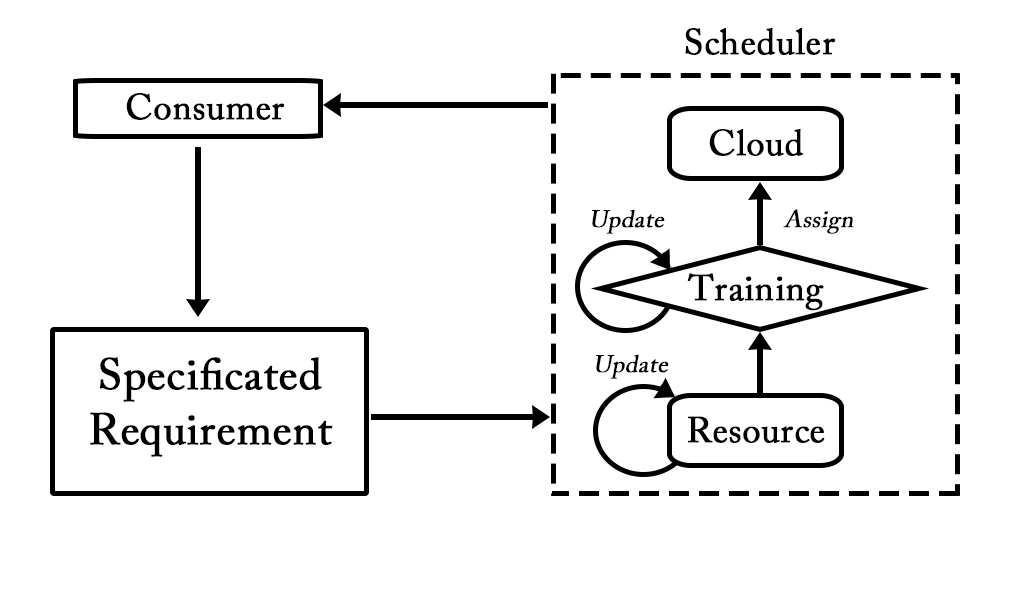
\includegraphics[width=1.0\textwidth]{Intro2.jpg}
	\end{figure2}


	2. Cosumer
	
	
	
	3. Schedulering Process
	
	\begin{figure3}
	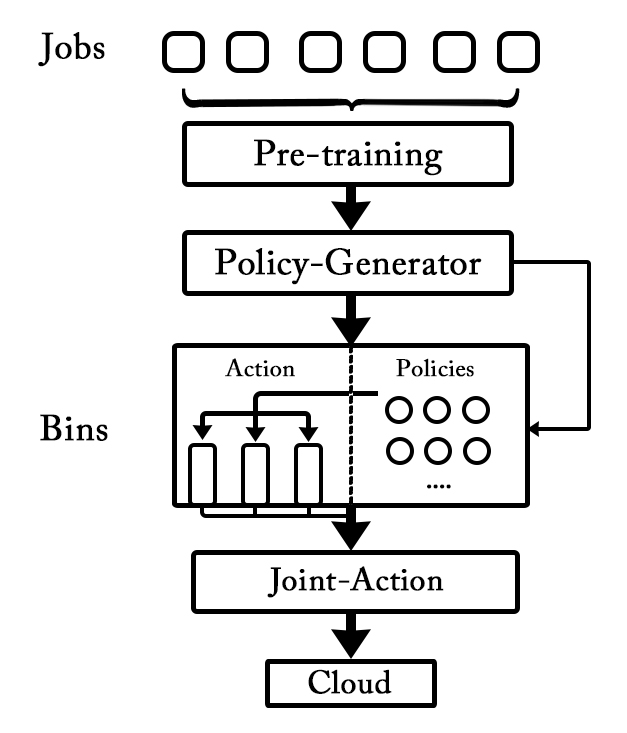
\includegraphics[width=1.0\textwidth]{Training2.jpg}
	\end{figure3}
	
		a. Pre-Traning
	
	\begin{figure4}
	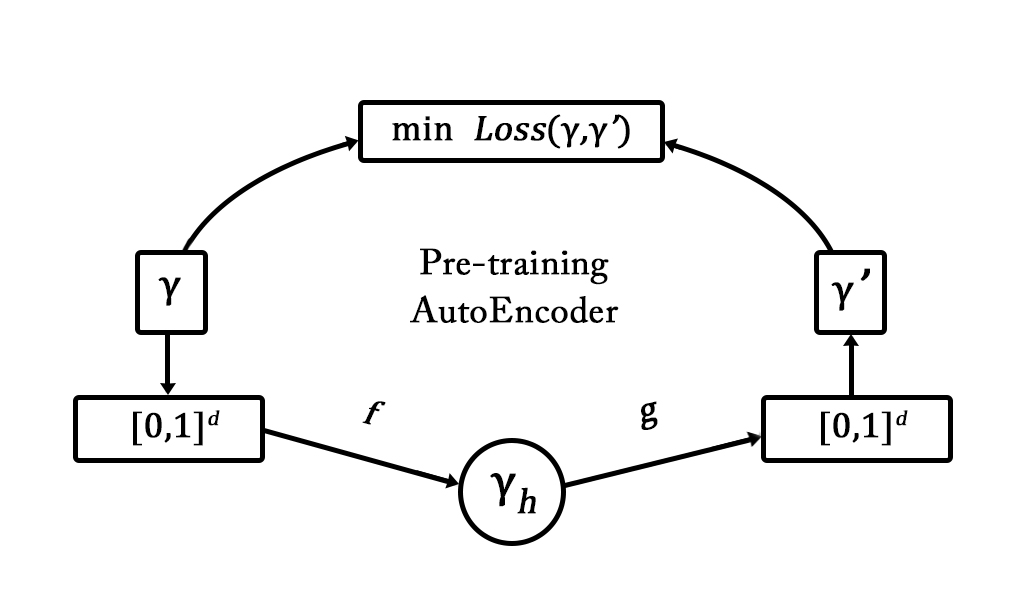
\includegraphics[width=1.0\textwidth]{Pre-Train.jpg}
	\end{figure4}
	
		b. Policy Generator
	
	\begin{figure5}
	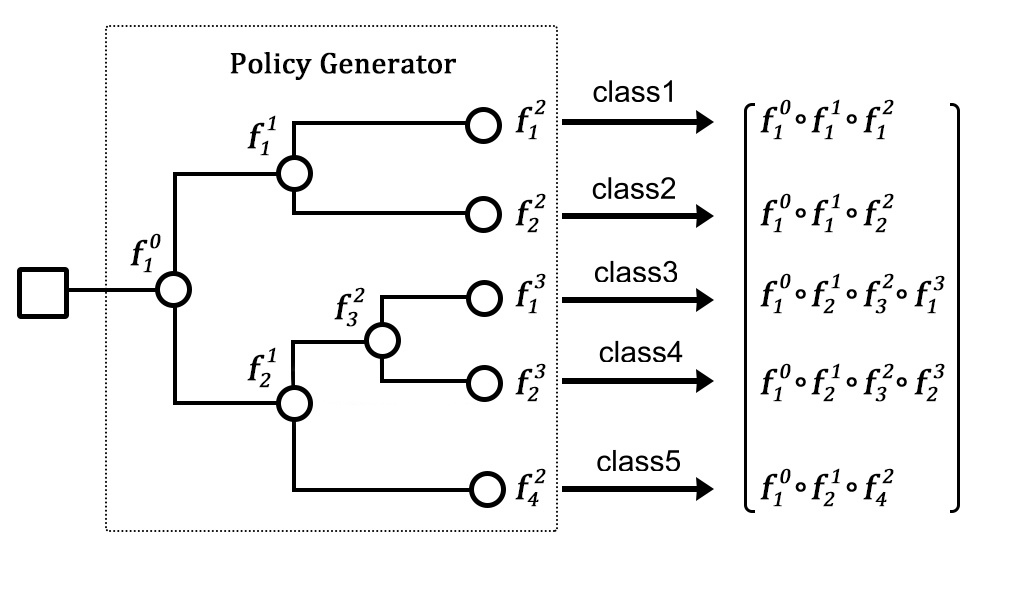
\includegraphics[width=1.0\textwidth]{Policy.png}
	\end{figure5}
	
	bayesian Hierarchical clustering
	
	c. Bins
	
	 d. Joint Actions
	
	\begin{figure6}
	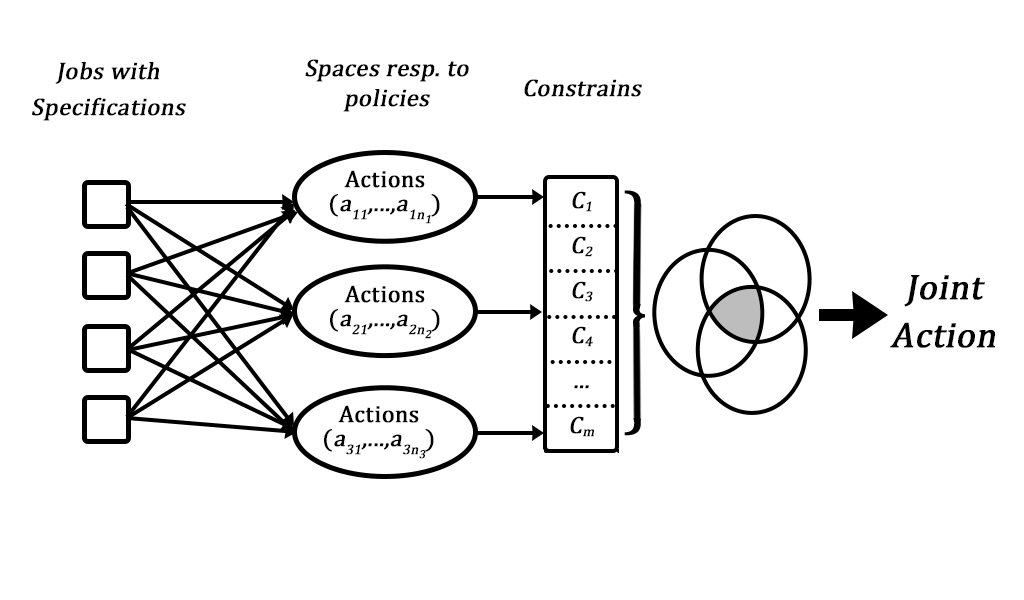
\includegraphics[width=1.0\textwidth]{Joint-action.jpg}
	\end{figure6}
	
	
	
	
	
	4. 
	
	\newpage
	
	\part{Consumers, Requirements and Specifications}
	
	\section{Consumer}
	
		\begin{definition}
			A \emph{consumer}, $c$, is a triple $(k, \phi, t)$, where $k \in \mathbb{N}$, $\phi$ is a specification, and $t \in \mathbb{R}^{+}$. The consumer $C$ is the subset of consumer $c$ which defined such that:
			\[
			c = (\phi , \sigma_m)
			\]
			\[
			C = 2^{\phi}*[0,\sigma_m)
			\]
		\end{definition}
		
		\begin{definition}
			Let \emph{service} $v$ be the available resource can be provide which related with a subset of resource $R'$ and a boolean variable $\beta$ can be defined such that:
			\[
			v := (R', \beta)
			\]
			\[
			V = 2^{R}*{\ss}
			\]
		\end{definition}
	
	\section{Requirements}
	
		\begin{definition}
			A \emph{requirement} is a function $\reqfunc{\rho}{X}$, where $X$ is a set and $\mathbb{B} = \{0,1\}$. The set $X$ is referred to as the required set of $\rho$.
		\end{definition}
		
		\begin{definition}
			A requirement $\rho$ is said to be \emph{separable} if and only if it may be written as $\rho(x) = \prod_{i \in I}{\rho_{i}(x)}$, where $\forall i \in I$, $\rho_{i}(x)$ is a requirement with required set $X$.
		\end{definition}
		
		\begin{definition}
			A \emph{requirement operator} is a mapping, $\mathbf{Req}: \mathbf{Set} \rightarrow \mathbf{Set}$, such that: \[\reqop{\rho}{X} := \setbuild{x}	{X}{\rho(x) = 1}.\]
		\end{definition}
		
		\begin{proposition}
			Given a requirement $\rho = \rho_{1}\cdot\rho_{2}$, where $\rho_{1}$ and $\rho_{2}$ are requirements with required set X, then: 
			\[
			\reqop{\rho}{X}\stackrel{~}{=}\reqop{\rho_{1}}{X}\cdot\reqop{\rho_{2}}{X}
			\]
		\end{proposition}
		
		\begin{remark}
			The binary operation $\cdot$ between two requirements is the same as the symbol, $\wedge$, used in boolean algebra to represent the join, $and$, between two boolean statements. Likewise, $\cdot$ operating on two sets is the intersection operation $\cap$. 
		\end{remark}
		
		\begin{proof}
			The proof of this proposition is very straightforward. Let $X$ be a set and $\rho$ be a requirement with required set $X$. Then,
			
			\begin{eqnarray}
			\reqop{\rho}{X} & = & \setbuild{x}{X}{\rho(x) = 1}\\ 
			& = & \setbuild{x}{X}{\rho_{1}(x)\cdot\rho_{2}(x) = 1}\\ 
			& = & \setbuild{x}{X}{\rho_{1}(x) = 1 \mathbin{and} \rho_{2}(x) = 1}\\ 
			& = & \setbuild{x}{X}{\rho_{1}(x) = 1}\cdot\setbuild{x}{X}{\rho_{2}(x) = 1}\\
			& = & \reqop{\rho_{1}}{X}\cdot\reqop{\rho_{2}}{X}
			\end{eqnarray}
		\end{proof}
	
	\section{Specifications}
	
		\begin{definition}
			A set, $X$, is said to be inspectable if and only if there exists a function, $\func{\psi}{X}{\prod_{i \in I}{X_{i}}}$, where $X \ne X_{i}, \forall i \in I$. This function is referred to as an \emph{inspection function} of $X$.
		\end{definition}
		
		\begin{remark}
			The inspection function may also be expressed as, $\psi(x) = (\psi_{i}(x))_{i \in I}.$
		\end{remark}
		
		\begin{definition}
			A \emph{specification} is a requirement, $\reqfunc{\phi}{X}$, such that the following conditions
			hold:
			
			\begin{enumerate}
				\item   The required set, $X$, is inspectable.
				
				\item   There exists a requirement, $\reqfunc{\varphi}{\prod_{i \in I}{X_{i}}}$,
				such that $\rho = \varphi \circ \psi$, where $\psi$ is an inspection function of $X$,
				with $X \ne X_{i}, \forall i \in I$. The requirement, $\varphi$, is referred to as an
				\emph{acceptance requirement} of X.
			\end{enumerate}
			
		\end{definition}
		
		\begin{theorem}
			Given a separable specification, $\phi$, with an acceptance requirement that is mutually independent,
			$\varphi(x_i)_{i \in I}$, then following isomorphism holds:
			
			\[
			\reqop{\phi}{X} = \prod_{i \in I}\reqop{\varphi_{i}}{X_{i}}
			\]
		\end{theorem}
	
	\newpage
	
	\part{Resources}
	
	\newpage
	
	\part{Scheduling Process}
	
	\section{Process Decomposition}
	
		\begin{definition}
			let $a$ represent the arriving process $a = (c, t_a)$. Then the assignment action A defined as:
			\[
			A = C * [0, \infty)
			\]
		\end{definition}
		
		\begin{definition}
			let $g$ represent the assignment process, $g = (c,\sigma_w, v)$. Then the assignment action G can be defined as:
			\[
			G = C*[0,\sigma_m)*V
			\]
		\end{definition}
		
		\begin{definition}
			let $d$ represent the departure process $d = (c, t_d)$, we also defined $\gamma(c) = min{\sigma_r,\sigma_m}.$ Then the departure action D defined as:
			\[
			D = C * [t_a, t_a + \sigma_w + \gamma(c)]
			\]
		\end{definition}
	
	\newpage
	
	\part{Reinforcement Model}
	
	\section{Policy Routing}
	
	\subsection{Policy Graph}
	
		\begin{definition} 
			Let $G = (V, E, src, tgt)$ be a graph. A \emph{path of length n} in $G$, denoted $p \in$ $\path{G}{(n)}$, is a head-to-tail sequence:
			\[
			p = (v_{1}   \labeledarrow{a_{1}}   v_{2}   \labeledarrow{a_{2}}  \cdots   \labeledarrow{a_{n-2}}  v_{n-1}   \labeledarrow{a_{n-1}}   v_{n})
			\]
			
			The \emph{set of all paths on G} is defined such that: 
			
			\[
			\pathall{G} : = \bigsqcup_{n \in \mathbb{N}}{\path{G}{(n)}}
			\]
		\end{definition}
		
		\begin{definition}
			let $\pathall{G}(v)$ be the all path from v back to v.
			
			The \emph{set of all path on G} is defined such that:
			
			$\pathall{G}(s,t) = \pathall{G}(s,v)\sqcup \cyclepath{G}(v) \sqcup \pathall{G}(v,t)$.
			
			The $\cyclepath{G}$ is defined as that:
			
			$\cyclepath{G}(v) = \pathall{G}(v,v)$
		\end{definition}
	
	\newpage    
	
\end{document}
